\documentclass[11pt]{article}
\usepackage{graphicx}
\usepackage{titling}
\usepackage{array}
\setcounter{secnumdepth}{0}
\usepackage{geometry}
\geometry{
	top=2cm,
}
\usepackage{hyperref}
\hypersetup{
	colorlinks=true,
	urlcolor=blue,
}
\urlstyle{same}

\preauthor{%
  \begin{center}
  \LARGE
  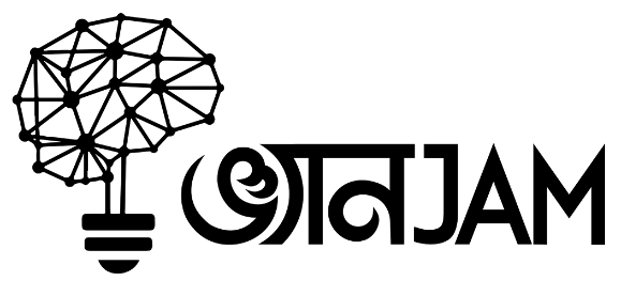
\includegraphics[scale=.4]{img/logo.png}\\[\bigskipamount]
}
\postauthor{\end{center}}
\title{Introduction to Machine Learning}
\date{}

\begin{document}
\maketitle
\section{Course Syllabus}
\begin{center}
\begin{tabular}{|m{1.15cm}|m{15cm}|}
\hline
Days &Topics\\ \hline
Day 0 & Machine Learning, Classifications of ML problems (Supervised, Reinforcement and Unsupervised) with examples\\ \hline
Day 1 & Tools for ML (Python, Conda, JupyterLab, Matlab), Python libraries for ML(SciPy, NumPy, Matplotlib, Pandas), Data visualization\\ \hline
Day 2 & Linear Algebra for ML, Cost function, Model and hypotheses representation, Gradient Descent, Linear regression\\ \hline
Day 3 & Classification and decision boundary, Logistic regression, Multiclass classification, Bias and Variance, Regularization\\ \hline
Day 4 & Deep Learning and Neural Networks, Logic gates with NN, Multiclass classification with NN\\ \hline
Day 5 & Neural Networks learning representation, Cost function, forward propagation, back-propagation, applications of NN\\ \hline
Day 6 & Learning curves, Training/Test/Cross Validation sets, Error Metrics (Precision, Recall, F1 Score), Confusion matrix, K-fold improvement\\ \hline
Day 7 & Large Margin classifiers, Kernels, Support Vector Machines, Decision Trees\\ \hline
Day 8 & Unsupervised learning algorithms, K-means clustering, Dimensionality reductions and Principal Component Analysis\\ \hline
Day 9 & Linear Discriminant Analysis, K-Nearest Neighbors\\ \hline
Day 10 & Gaussian Distribution, Multi-variate Gaussian Distribution, Anomaly Detection, Recommender Systems\\ \hline
Day 11 & Online learning, Batch Gradient Descent, Map-reduce and Data parallelism, Multi-core workload distribution\\ \hline
\end{tabular}
\end{center}
\end{document}